%--------------------Projet3---------------
%--------------------Marrakech-------------
%-----Created: 05/07/2019-----------------
%-----Last modification: 05/07/2019--------

\documentclass [reqno]{amsart}
\usepackage[english]{babel}
\usepackage{textcomp}
\usepackage[leqno]{amsmath}
\usepackage{amsfonts,amssymb,amsthm,mathrsfs,float}
\usepackage{lmodern}
\usepackage{hyperref}
\usepackage{etoolbox}
\usepackage{mathptmx}
\usepackage{cancel}
\usepackage{graphicx}
\graphicspath{ {./images/} }
\patchcmd{\abstract}{\scshape\abstractname}{\textbf{\abstractname}}{}{}
\hypersetup{urlcolor=blue, colorlinks=true, citecolor=blue}  % Colours hyperlinks in blue, but this can be distracting if there are many links.
%\usepackage{cite}
%\renewcommand{\citeleft}{\textcolor{blue}{[}}
%\renewcommand{\citeright}{\textcolor{blue}{]}}
%partie réelle d'un complexe
\renewcommand{\Re}{\operatorname{Re}}
%partie imaginaire d'un complexe
\renewcommand{\Im}{\operatorname{Im}}

\DeclareGraphicsExtensions{.png,.pdf,.eps,.jpg}
%openin
\title[{\tiny Uniform exponential and polynomial stabilty and approximation in control of a thermoelastic model}]{
 \bf Uniform exponential and polynomial stabilty and approximation in control of a thermoelastic model}
%\author{L. Maniar, S. Nafiri}
 %in alphabetical order

%\address{Lahcen Maniar \newline
%Departement de Mathematiques, Faculte des Sciences Semlalia, Universite Cadi Ayyad, B.P. 2390, 40000 Marrakesh, Morocco.}
%\email{lahcenmaniar@gmail.com}
%
%\address{Salem Nafiri \newline
%Departement de Mathematiques, Faculte des Sciences Semlalia, Universite Cadi Ayyad, B.P. 2390, 40000 Marrakesh, Morocco.}
%\email{nafirisalim@gmail.com}

\date{}
\raggedbottom %no extra vertical spaces is added
\begin{document}
\maketitle
\numberwithin{equation}{section}
\newtheorem{thm}{Theorem}[section]
\newtheorem{lem}{Lemma}[section]
\newtheorem{prop}{Proposition}[section]
\newtheorem{Def}{Definition}[section]
\newtheorem{rmk}{Remark}[section]
%\newtheorem*{dem}{Proof}
\newenvironment{dem}{\noindent\textbf{Proof.~}}{\hfill$\square$\bigbreak}

\section*{\bf Model Problem}
We consider the numerical approximation of the following coupled thermoelastic wave models
\begin{equation}
\label{eq1}
\tag{1}
 \left\{\begin{array}{llll}
                      u_{tt}(x,t)- \Delta u(x,t)+\gamma\theta_x(x,t)=0\quad &in\;\Omega\times(0, \infty)\\
		      \theta_{t}(x,t)-\Delta\theta(x,t)-\gamma u_{tx}(x,t) =0\quad &in\;\Omega\times(0, \infty)\\
		      u(x,t)=0=\theta(x,t)\qquad &\text{on } \partial\Omega\times(0,\infty)\\
u(x,0)=u_{0}(x),\; u_{t}(x,0)=u_{1}(x),\; \theta(x,0)=\theta_{0}(x) \quad &on \;\Omega
                     \end{array}
                   \right.
\end{equation}

\begin{equation}
\label{eq2}
\tag{2}
 \left\{\begin{array}{llll}
                      u_{tt}(x,t)- \Delta u(x,t)+\gamma\theta(x,t)=0\quad &in\;\Omega\times(0, \infty)\\
		      \theta_{t}(x,t)-\Delta\theta(x,t)-\gamma u_{t}(x,t) =0\quad &in\;\Omega\times(0, \infty)\\
		      u(x,t)=0=\theta(x,t)\qquad &\text{on } \partial\Omega\times(0,\infty)\\
u(x,0)=u_{0}(x),\; u_{t}(x,0)=u_{1}(x),\; \theta(x,0)=\theta_{0}(x) \quad &on \;\Omega
                     \end{array}
                   \right.
\end{equation}
where $u(x,t)$ is the displacement (longitudinal or transverse, depending upon the application) at position $x$ along a bounded smooth domain $\Omega\subset\mathbb{R}$ and time $t$ , and $\theta(x,t)$ is the temperature deviation from the reference temperature at position $x$ and time $t$, $u_0(x)$, $v_0(x)$ and $\theta_0(x)$ are initial data in a suitable space. The small positive constant $\gamma$ is a thermo-mechanical coupling parameter and is generally small in comparison to 1. System (\ref{eq1}) differs from system (\ref{eq2}) at the coupling terms, where we have replaced the strong coupling ($\gamma\theta_x$ and $\gamma u_{tx}$) by a weak coupling ($\gamma\theta$ and $\gamma u_{t}$).
It is well known from literature that system (\ref{eq1}) and (\ref{eq2}) are respectively exponentially and polynomially stable, see \cite{Hansen1992, LZb1993} and \cite{KBT1997, KBB1999, LR2005}.

In this post, we will show by numerical experiments, how the coupling terms affect quantitative and qualitative properties of thermoelastic systems $\eqref{eq1}$ and $\eqref{eq2}$. These results could be found in \cite{LZb1994,MN2016}.

To do this, we consider a semi discretization version of both systems $\eqref{eq1}$ and $\eqref{eq2}$, obtained with finite element method, which has the following form
\begin{equation}
\label{eq3}
\tag{3}
 (S_i)\left\{\begin{array}{ll}
 z'_n(t)=A_{i,n} z_n(t),\quad t\geq 0,\;n\in\mathbb{N},\;i=1,2\\
 z_n(0)=z_{n0},\;n\in\mathbb{N}\\
\end{array}
\right.
\end{equation}
where for all $n\in\mathbb{N}$, $z_n=(u_n,v_n,\theta_n)^T$ is the semi discrete solution, $z_{n0}$ is the discretized initial data, $A_{i,n}$ the discretized dynamic and the subscript $\cdot_i$ refers to system $\eqref{eq1}$ and $\eqref{eq2}$ with  
\begin{align*}
A_{i,n}=\left(\begin{matrix}
                    0 & D_n & 0\\
	       -D_n & 0 & -\gamma F_{i,n}\\
		    0 & \gamma F_{i,n} & -D_n^2
                   \end{matrix}
\right),\quad i=1,2
\end{align*}
and $F_{2,n}=I_n$, 
\begin{align*}
D_n=\left(\begin{matrix}
                    1 &  & \\
	        & \ddots &  \\
		     &   & n
                   \end{matrix}
\right),\quad (F_{1,n})_{ij}=\left\{\begin{array}{ll}
 -\frac{4}{\pi}\frac{ij}{i^2-j^2},\quad |i-j|=\text{odd},\\
 0,\qquad\qquad\text{otherwise}.
\end{array}
\right.
\end{align*}

\section*{\bf Spectral properties of thermoelastic systems}

Figure 1 and Figure 2 show how the coupling terms affect the placement of eigenvalues of the dynamic $A_{n}$. In Figure 1, we see that a uniform distance between the eigenvalues and the imaginary axis is preserved, see Table 1. Another observation is that for fixed $n$, the eigenvalues of higher frequency modes, in particular, the one of the $n^{th}$ mode, are closer to the imaginary axis. Moreover, as the number of modes increases, these eigenvalues bend back towards the vertical line $\lambda=-\frac{\gamma^2}{2}$, a fact which has been already shown in \cite{KBT1996}. Therefore, the corresponding spectral element approximation scheme preserves the property of exponential stability.
\begin{table}[H]
\begin{center}
\caption{Distance between $\sigma(A_{1,n})$ and the imaginary axis for the spectral element method}
\begin{tabular}{|c|c|} 
\hline
n & min\{-Re$\lambda$, $\lambda\in\sigma(A_{1,n})$\}\\
\hline 
8 & 8.9227$\times 10^{-4}$\\
\hline
16 & 8.9383$\times 10^{-4}$\\
\hline
24 & 8.9402$\times 10^{-4}$\\
\hline
32 & 8.9407$\times 10^{-4}$\\ 
\hline
\end{tabular}
\end{center}
\end{table}
\begin{figure}[H]
\label{fig1}
\begin{center}
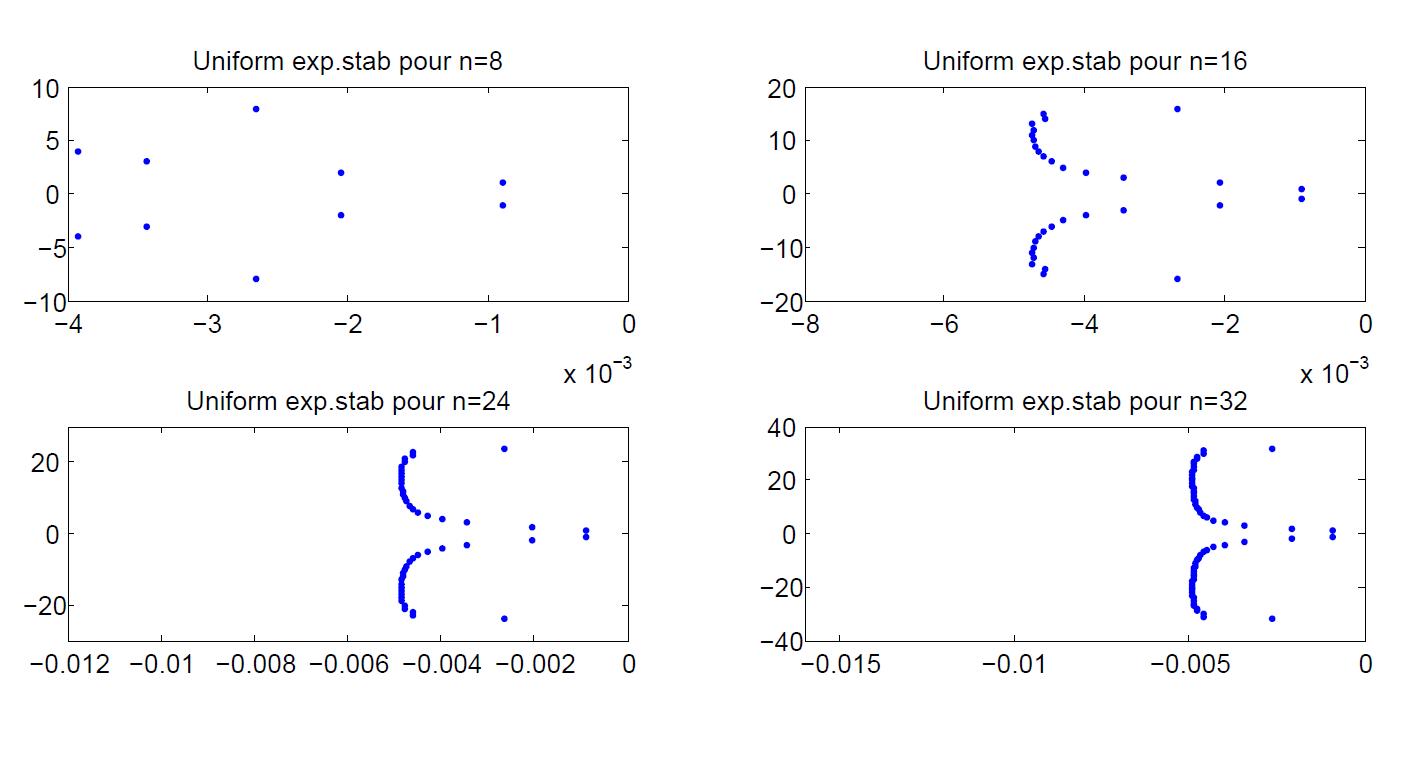
\includegraphics[scale=0.4]{spec_exp_thermo}
\caption{Location of the complex eigenvalues of the matrix $A_{1,n}$ with the finite element method}
\end{center}
\end{figure}
In Figure 2, conversely to Figure 1 where a uniform distance between the eigenvalues and the imaginary axis is preserved, we observe that, as the number of modes increases, an asymptotic behaviour appears in the neighborhood of the imaginary axis at $\pm\infty$. This property is mainly related to systems with polynomial decay, see \cite{BEPS2006}.
\begin{figure}[H]
\begin{center}
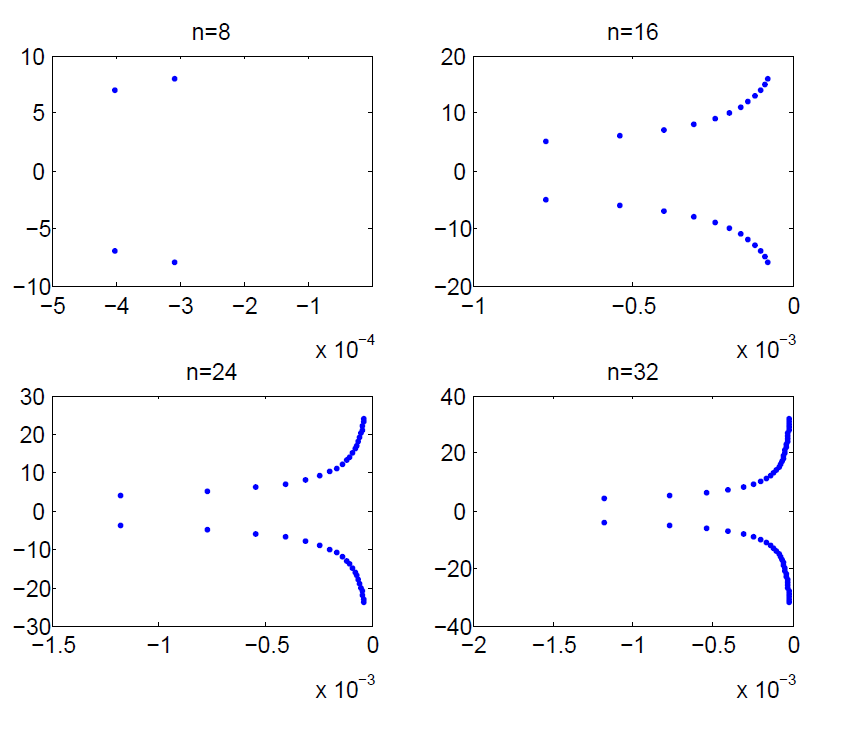
\includegraphics[scale=0.5]{spec_poly_thermo}
\caption{Location of the complex eigenvalues of the matrix $A_{2,n}$ with the finite element method.}
\end{center}
\end{figure}
\section*{\bf Uniform and polynomial decay of the energy}
The discrete energy associated to system \eqref{eq3} is given by
\begin{equation}
\label{eq4}
\tag{4}
E_{i,n}(t)=\frac{1}{2}\sum_{j=1}^n\Big\{|u_j(t)|^{2}+|v_j(t)|^{2}+|\theta_j(t)|^{2}\Big\},\;i=1,2.
\end{equation}
The discrete energy $E_{1,n}$ associated to system $\eqref{eq1}$ decays exponentially to zero, see Figure 3, in the following sense: $\exists M,\alpha$ positive constants such that
\[
E_{1,n}(t)\leqslant Me^{-\alpha t}E_{1,n}(0),\;n\in\mathbb{N},\;t>0.
\]
However, the introduction of the weak coupling term in system $\eqref{eq1}$ has changed the dynamic and consequently the behavior of energy \eqref{eq4}. In this case, we say that system \eqref{eq2} decays polynomially to zero, see Figure 4, in the following sense: $\exists M,\alpha$ positive constants such that
\[
E_{2,n}(t)\leqslant \frac{M}{t}\|A_{2,n}z_{n0}\|^2,\;n\in\mathbb{N},\;t>0.
\]
\begin{figure}[H]
\begin{center}
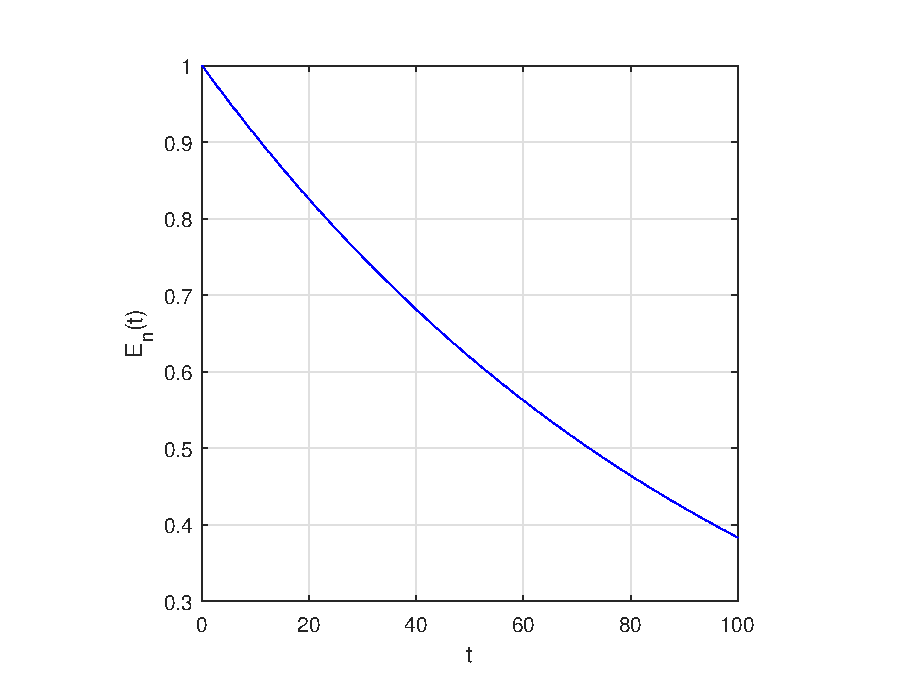
\includegraphics[scale=0.8]{exp}
\caption{Exponential decay of $E_{1,n}(t)$}
\end{center}
\end{figure}
\begin{figure}[H]
\begin{center}
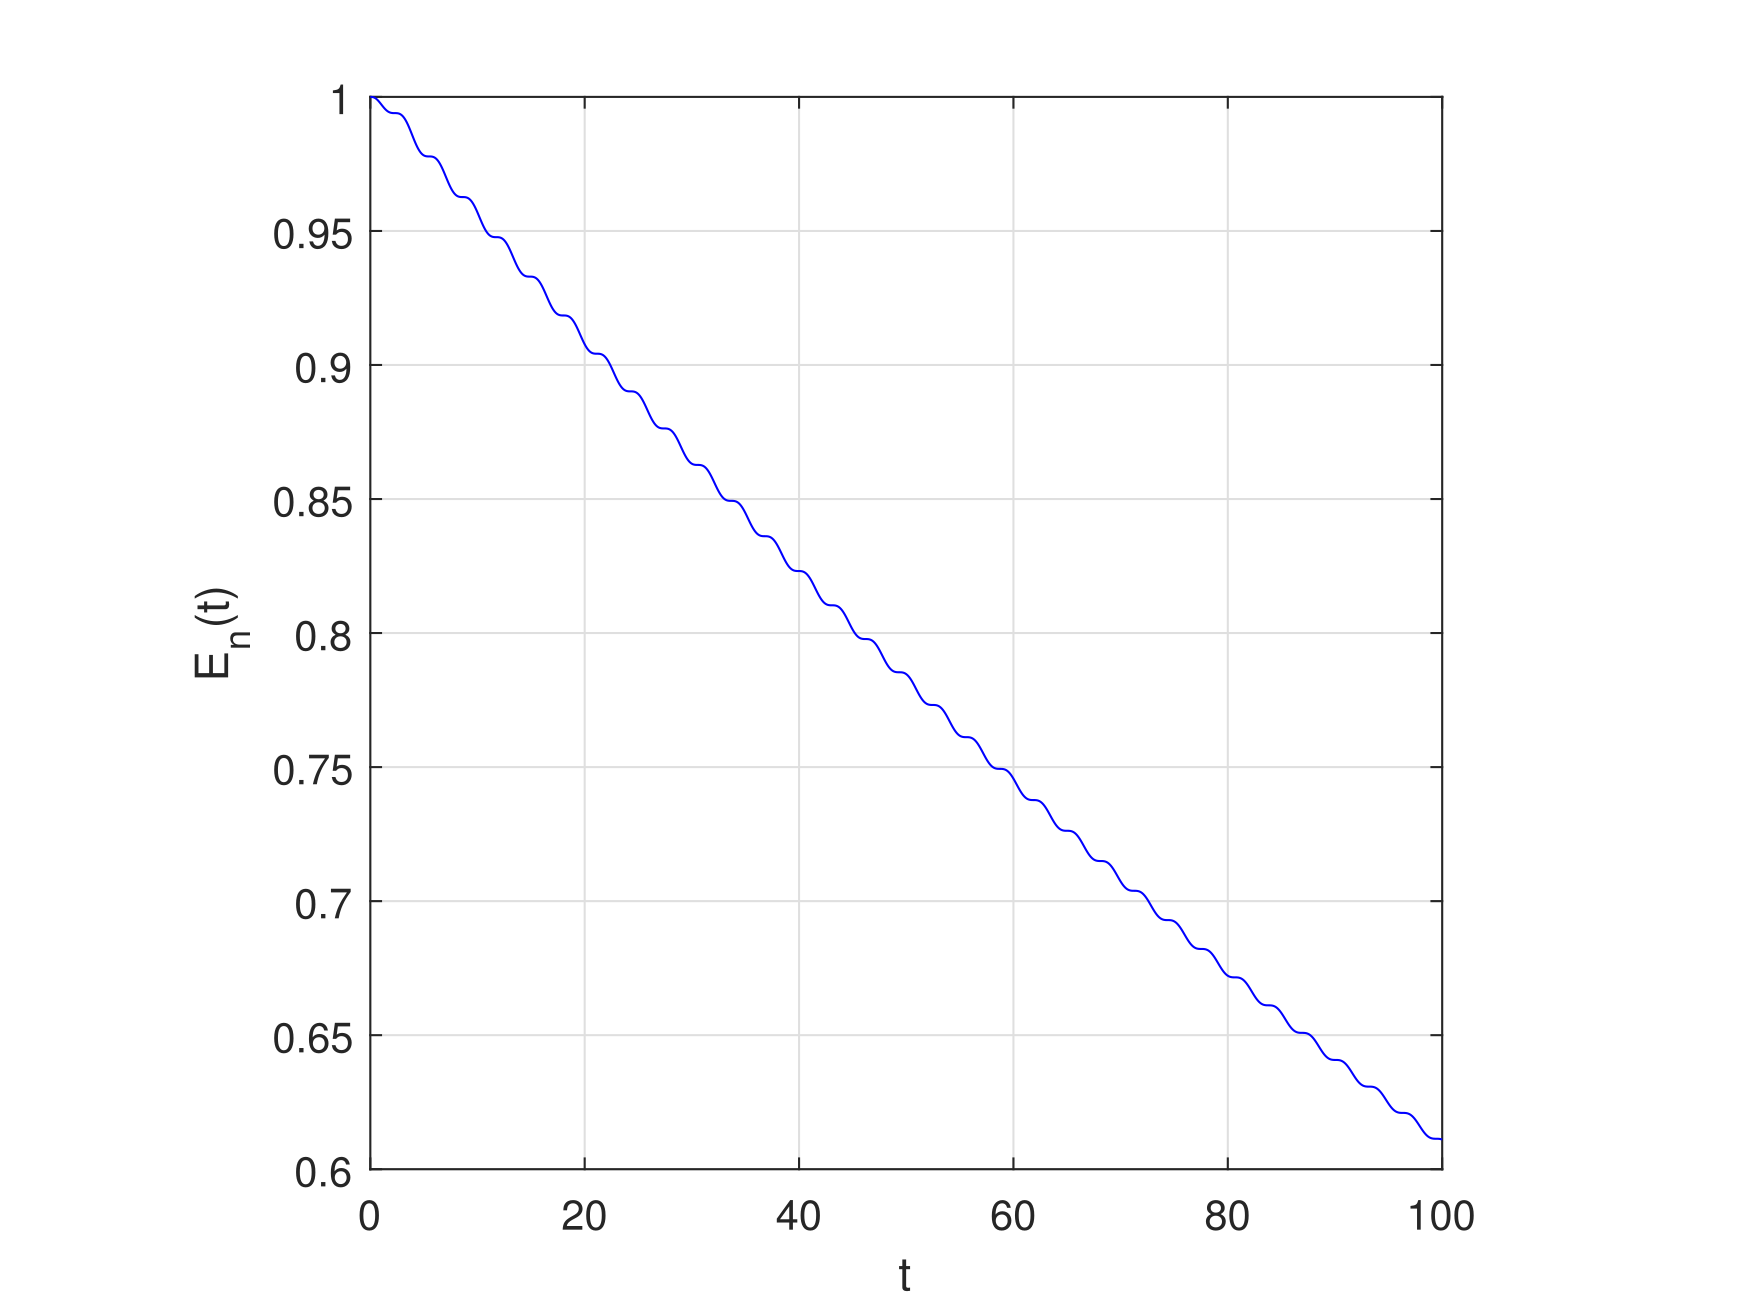
\includegraphics[scale=0.8]{poly}
\caption{Polynomial decay of $E_{2,n}(t)$}
\end{center}
\end{figure}

\section*{\bf Effect of smoothness of the initial data on the rate of decay of energy} 
It has been shown theoretically, see \cite{BEPS2006, BT2010}, that the energy associated to system \eqref{eq2} is very sensitive to the smoothness of its initial data. This fact, has been also observed numerically, see Figure 6. 
we use a uniform mesh with $n = 100$ elements, fix the final time at $T = 100$, use dt = 0.1 and consider the following initial conditions for $u$ $u_t$ and $\theta$
\[
u(x,0) = 0,\quad \theta(x, 0) = 0,\quad u_t(x, 0) =sin(jx),\; j = 1, 2, 3.
\]
Through Figure 6, we notice that for $j = 1$, the approximate energy $E_{2,n}(t)$ decays to zero as the time $t$ increases. Moreover, we observe that the decay rate depends strongly to j. That is, when $j$ increases, initial data are very oscillating. We say in this case that the rate of decay of the discrete energy $E_{2,n}(t)$ is very sensitive to
the choice of the initial data. However, the behavior of the energy assosiated to system \eqref{eq1} remains indifferent to the smoothness of initial data when $n\to\infty$, see Figure 5.
\begin{figure}[H]
\begin{center}
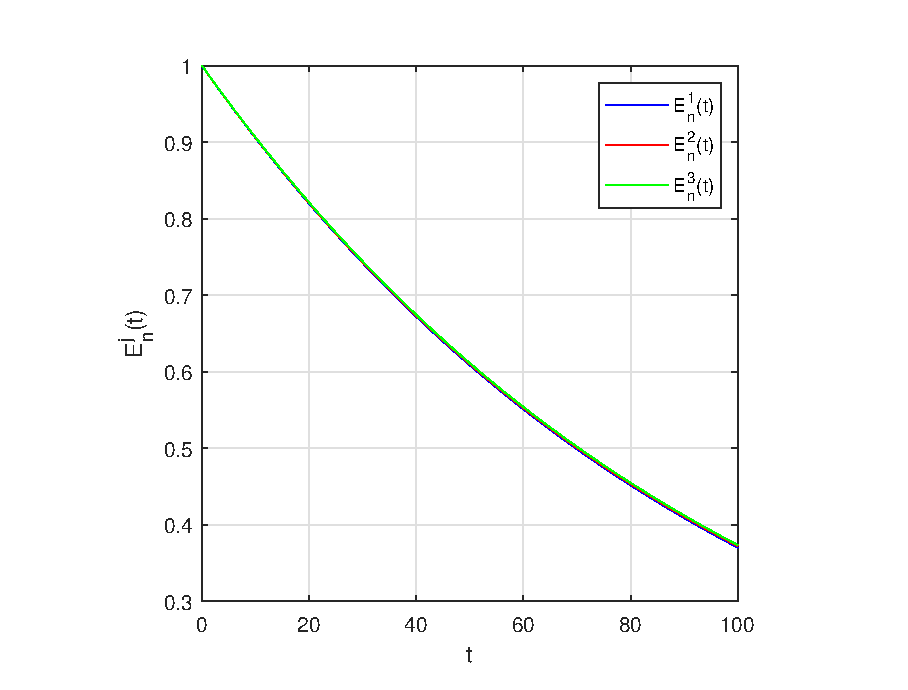
\includegraphics[scale=0.8]{fig5}
\caption{No effect of smoothness on exponential decay of $E_{1,n}(t)$}
\end{center}
\end{figure}
\begin{figure}[H]
\begin{center}
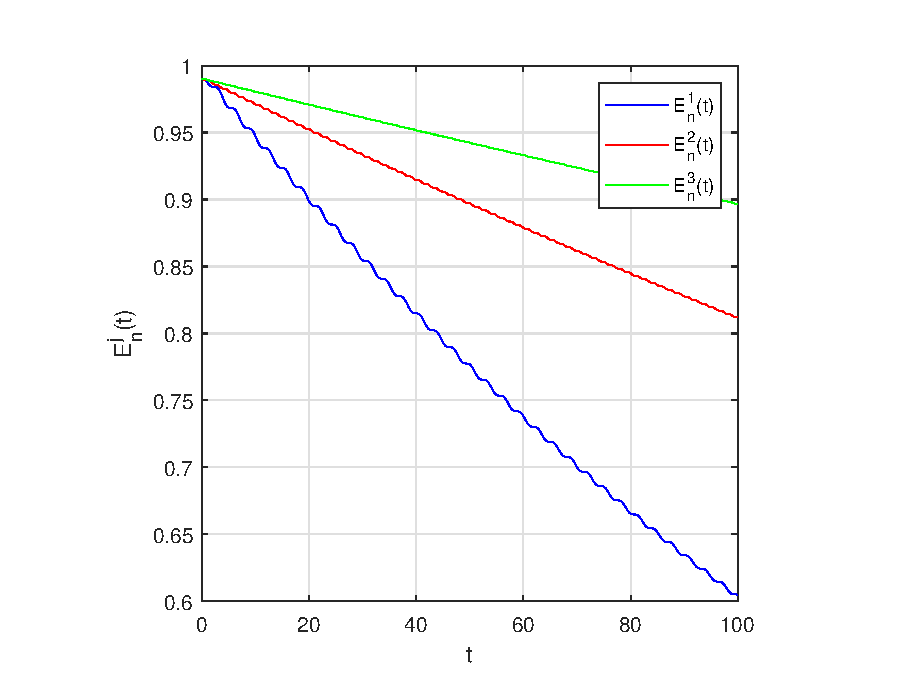
\includegraphics[scale=0.8]{fig6}
\caption{Effect of smoothness on polynomial decay of $E_{2,n}(t)$}
\end{center}
\end{figure}
\begin{thebibliography}{00}

\bibitem{BEPS2006} A. B\' atkai, K.J. Engel, J. Pr\"uss and R. Schnaubelt, \textit{Polynomial stability of operator semigroups}, Math. Nachr. 279 (2006) pp. 1425–1440.

\bibitem{BT2010} A. Borichev and Y. Tomilov, \textit{Optimal polynomial decay of functions and operator semigroups}, Math. Ann., 347(2), pp.455-478,2010.


\bibitem{Hansen1992} S. W. Hansen, \textit{Exponential energy decay in a linear thermoelastic rod}. J. Math. Anal. Appli.,\textbf{167}, 1992, pp. 429-442.

\bibitem{KBT1996} F.A. Khodja, A. Benabdallah, and D. Teniou, \textit{Stability of coupled systems}, Abstr. Appl. Anal. Volume 1, Number 3(1996), 327-340.

\bibitem{KBT1997} F. A. Khodja, A. Benabdallah and D. Teniou, \textit{Dynamical stabilizers and coupled systems}, ESAIM Proceeding, \textbf{2}, (1997), pp. 253-262.

\bibitem{KBB1999} F. A. Khodja, A. Bader and A. Benabdallah, \textit{Dynamic stabilization of systems via decoupling techniques}, ESAIM: COCV, \textbf{4}, (1999), 577–593.

\bibitem{LZb1993} Z. Liu and S. Zheng, \textit{Exponential stability of semigroup associated with thermoelastic system}, Quart. Appl. Math, 51, (1993), pp. 535-545.

\bibitem{LZb1994} Z. Y. Liu and S. Zheng, \textit{Uniform exponential stability and approximation in control of a thermoelastic system}, SIAM J. Control Optim. 32, (1994), pp.
1226-1246.

\bibitem{LR2005} Z. Liu and B. Rao, \textit{Characterization of polynomial decay rate for the solution of linear evolution equation}. Zeitschrift f\"ur angewandte Mathematik und Physik ZAMP, \textbf{56}, (2005), pp. 630-644.

\bibitem{MN2016} L. Maniar and S. Nafiri, \textit{Approximation and uniform polynomial stability of $C_0-$semigroups}, ESAIM: COCV 22, 2016, pp. 208-235.

\end{thebibliography}
\end{document}

\bibitem{Hu1985} F. L. Huang, \textit{Characteristic conditions for exponential stability of linear dynamical systems in Hilbert spaces}, Ann. Diff. Eq. \textbf{1}, (1985), pp. 43-56.



\bibitem{JLions1988} J. L. Lions, \textit{Contrôlabilité exacte, Perturbations et Stabilisation de Systèmes Distribués}, Vol \textbf{1} et \textbf{2}, R.M.A. 9, Masson (1988).



\bibitem{LZb1999} Z. Y. Liu and S. Zheng, \textit{Semigroups Associated with Dissipative Systems}. Chapman \& Hall/CRC Research Notes in Mathematics Series (1999).



\bibitem{Nowacki1970} W. Nowacki, \textit{Problems of thermoelasticity}, Progress in Aerospace Sciences, Polskiej Akademie Nauk, Warszawa, \textbf{10}, (1970), pp. 1–63.

\bibitem{Pazy1983} A. Pazy, \textit{Semigroups of linear operators and applications to partial differential equations}, Applied Math. Sciences, \textbf{44}, Springer-Verlag, New York (1983).

\bibitem{P1984} J. Pr\" uss, \textit{On the spectrum of $C_{0}$-semigroups}. Transactions of the American Mathematical Society, (1984), \textbf{284}, pp. 847–857.

\bibitem{R1992}J. E. M. Rivera, \textit{Energy decay rate in linear thermoelasticity}, Funkcial. Ekvac. \textbf{35}, (1992), pp. 19-30.

\bibitem{Walker1980} J. A. Walker, \textit{Dynamical Systems and Evolution Equations: Theory and Applications}, \textbf{20} of Mathematical Concepts and Methods in Science and Engineering. Plenum, 1980.

\bibitem{AB1988} W. Arendt and C. J. K. Batty, \textit{Tauberian theorems and stability of one parameter semigroups}, Trans. Amer. Math. Soc.,306 (2), pp. 837–852, 1988.

\bibitem{BD2008} C. J. K. Batty and T. Duyckaerts, \textit{Non-uniform stabilityfor bounded semigroups on Banach spaces}, J. Evol. Equ., 8(4), pp.765-780, 2008.

\bibitem{B1978} C.D. Benchimol. \textit{A note on weak stabilizability of contraction semigroups}. SIAM J. Control. optim., \textbf{16}, pp. 373-379, 1978.

\bibitem{BT2010} A. Borichev and Y. Tomilov, \textit{Optimal polynomial decay of functions and operator semigroups}, Math. Ann., 347(2), pp.455-478,2010.

\bibitem{Dafermos1968} C. M. Dafermos, \textit{On the existence and the asymptotic stability of solutions to the equations of linear thermoelasticity}. Arch. Rat. Mech. Anal., \textbf{29}, (1968), pp. 241-271.

\bibitem{EN2000} K. Engel and R. Nagel, \textit{One-parameter semigroups for linear evolution equations}. Encyclopedia of Mathematics and its Applications. Springer-Verlag, New York, 2000.

\bibitem{G1978} L. Gearhart, \textit{Spectral theory for contraction semigroups on Hilbert space}. Transactions of the American Mathematical Society, (1978), \textbf{236}, pp. 385-394.

\bibitem{G1967} P. Grisvard, \textit{Caracterization de quelques espaces d'interpolation}, Arch. Rational Mech. Anal.,25 (1967), pp. 40-63.
